\chapter{Verwandte Arbeiten}
\label{chap:VerwandteArbeiten}

Im Zuge unserer Recherche zu Multi-Wan Bonding sind wir auf verschiedene bereits existierende Hardware-/ und Software-Lösungen gestoßen, welche wir uns in diesem Kapitel genauer Ansehen werden. Die zwei Lösungen unterscheiden sich in drei wesentlichen Aspekten zum einen der Preis, die Flexibilität und die Anzahl der verschiedenen  Internetverbindungen. Der Preis bei den Hardware-Lösungen ist einmalig zu bezahlen, im Gegensatz zu den Software-Lösungen die mittels Abonnement zu bezahlen sind. Aus finanzieller Sicht sind also die Hardware-Lösungen besser. Die Hardware-Version ist jedoch nicht flexibel da man immer einen Router, Stromverbindung und Kabel haben muss, daher ist man sehr Ortsgebunden, das ist für Zuhause oder im Büro kein Problem. Aber, wenn man auch Unterwegs mehr als eine Internetverbindung nutzen möchte ist die Software-Lösung die einzige Option. Die Anzahl an verschiedenen Internetverbindungen ist bei den Hardware-Lösungen beschränkt, bei der Software-Lösung können das unendlich viele sein.

\section{VPN}

\begin{figure}[H]
    \centering
    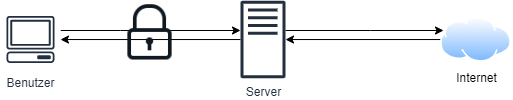
\includegraphics[width=0.8\textwidth]{VPN.png}
    \caption[VPN]{Virtual Private Network} 
\end{figure}

\section{Hardware-Lösungen}

\subsection{Multi-Wan Bonding Router}
Um einen Multi-Wan Bonding Router verwenden zu können werden mindesten zwei Router mit verschiedenen Internetanbindungen benötigt, die dann an den WAN-Ports des Multi-Wan Bonding Routers angeschlossen werden. Die Router besitzen zwei verschiedene Modi zum einen Loadbalancing welches beide Anbindungen maximal auslastet und Fallback, welches eine Internetanbindung voll ausnutzt, die zweite wird nur benutzt, falls die erste ausfällt.

\subsubsection{TP-Link Gigabit Ethernet Safestream VPN Router}
Mit diesem Router ist es möglich bis zu vier verschiedene Gigabit Internetanbindungen gleichzeitig zu nutzen. Das VPN im Namen steht dafür, das man sich mit dem Router zu einem VPN verbinden kann und somit alle Verbindungen im Netzwerk zu dem VPN-Server laufen. Dieser Router ist für 138,00 € auf Amazon erhältlich

\section{Software-Lösungen}

\subsection{Speedify}
Speedify ist eine bereits existierende Multi-Wan Bonding Software-Lösung, die das Benützen von mehreren Internetverbindungen gleichzeitig möglich macht. Es ist auch ein VPN. Bei Speedify sind nur 2 GB an Datenübertragung pro Monat kostenlos, wenn man mehr Datenvolumen benötigt muss man sich für ein kostenpflichtiges Abonnement entscheiden. Es gibt 3 verschiedene Abonnements bei denen sich die Anzahl an Nutzern verändert, je Nutzer kann man Speedify auf bis zu 5 Geräten gleichzeitig nutzen.
\begin{itemize}
    \item Für Einzelpersonen um 9.99 USD inkludiert 1 Benutzerkonto
    \item Für Familien um 14.95 USD mit 5 Benutzerkonten
    \item Für Firmenkunden um 9.99 USD pro Person
\end{itemize}
\  \\
Unsere Lösung ist im Gegensatz zu Speedify Open-Source und komplett kostenlos. Das einzige das von einem Benutzer benötigt wird, ist ein Server mit einer guten Internetanbindung, sowohl der Upload als auch der Download sind dabei wichtig.

\subsection{OpenVPN}
OpenVPN ist eine Open-Source VPN-Lösung, die es einem möglich macht seine Verbindung zu verschlüsseln, dazu wird OpenSSL oder mbed TLS verwendet. Viele kommerzielle VPNs zum Beispiel NordVPN und Surfshark basieren auf OpenVPN.
\newline
\newline
OpenVPN unterstützt kein Multi-Wan Bonding deshalb kann es nicht als Alternative oder Konkurrenz angesehen werden.
